\chapter{Vetores}
Com os conhecimentos até o momento caso seja necessário mais de uma variável que faça a mesma função deve-se declarar cada uma delas separadamente, porém há uma maneira de guardar estas variáveis em posições sequenciais de memória como mostra a Figura \ref{fig:memVetor}.
\begin{figure}[!h]
    \centering
    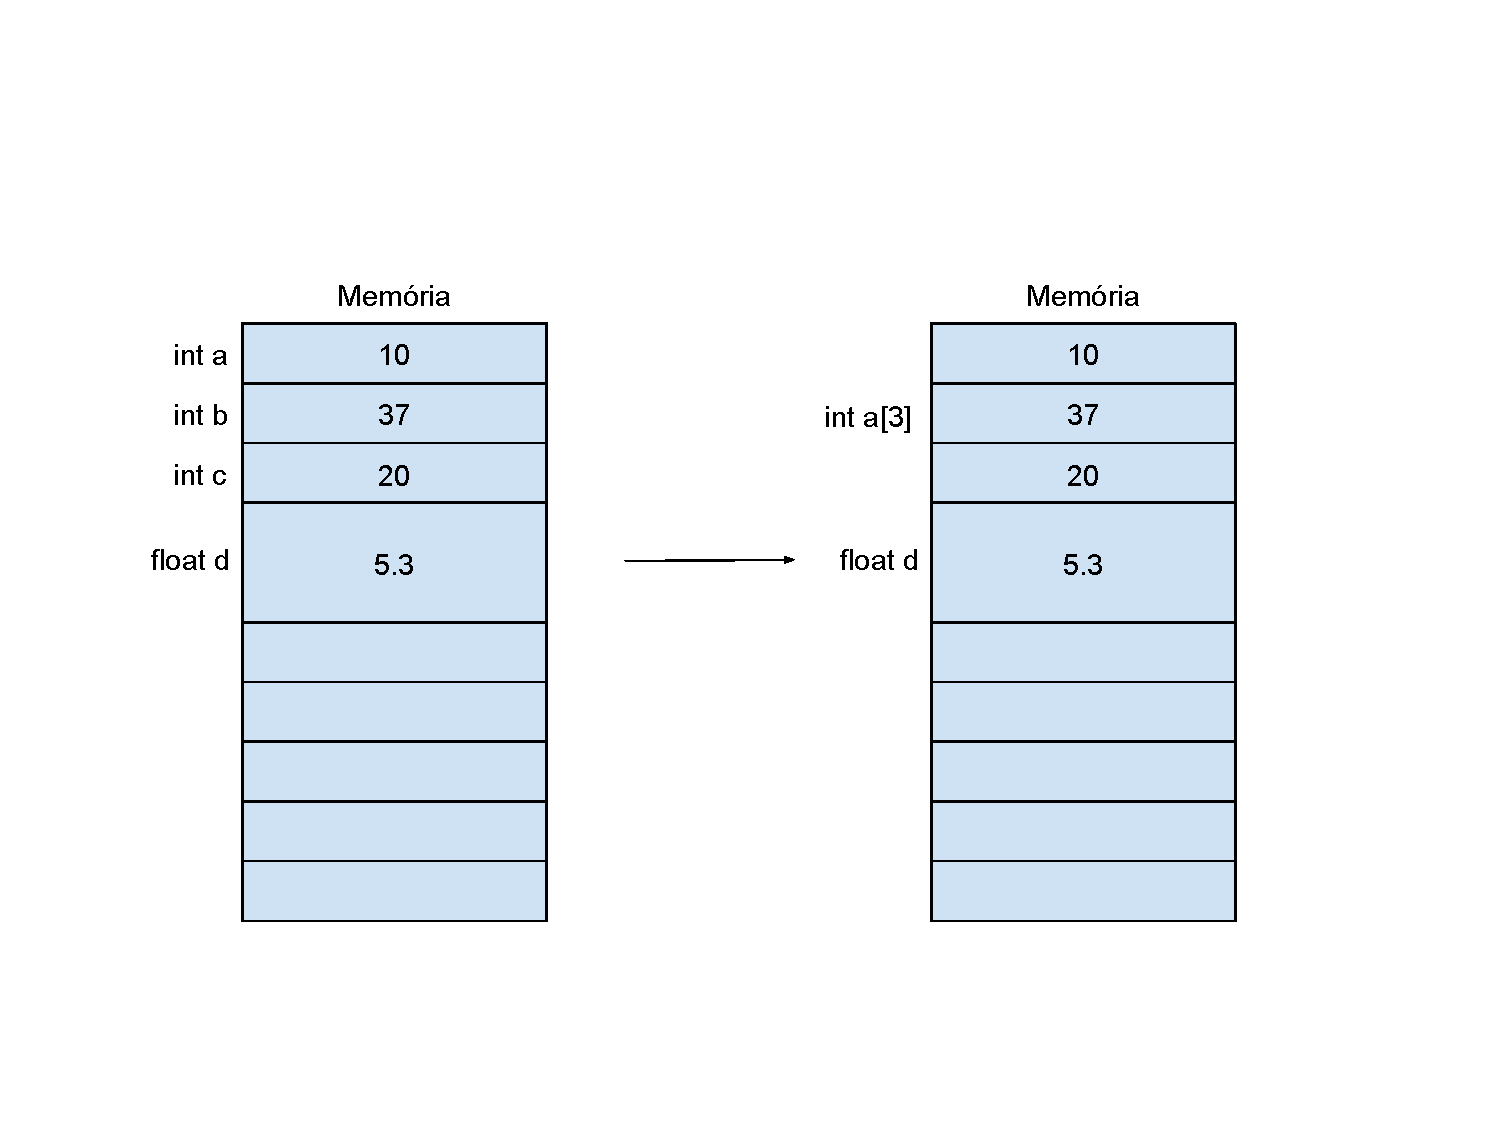
\includegraphics[scale=.5]{memVetor.pdf}
    \caption{Alocação de memória para vetores}
    \label{fig:memVetor}
\end{figure}
Desta forma o acesso as variáveis em vetor, considerando o exemplo da figura se dá por a[0] para o primeiro, a[1] para o segundo e a[2] para o terceiro, totalizando três variáveis inteiras. Considere agora que nestas três posições estejam o salário de funcionários de uma empresa e que eles receberam um aumento de 10\%, previamente precisaria-se de algo do tipo:
\begin{lstlisting}
    salario0,salario1,salario2,...,salarioN: inteiro
    Leia(salario0,salario1,salario2,...,salarioN)
    salario0 = salario0 * 1.1
    salario1 = salario1 * 1.1
    salario2 = salario2 * 1.1
    .
    .
    .
    salarioN = salarioN * 1.1
\end{lstlisting}
Note que precisaria-se de $N$ linhas para $N$ funcionários, portanto o código ficaria bem extenso, porém, pode-se utilizar uma estrutura de repetição junto de um vetor para facilitar o trabalho:
\begin{lstlisting}
    N: inteiro
    N = 10
    salario: vetor [N] de inteiro
    #Le os salarios de cada funcionario
    Para i = 0 ate N em passos de 1 faca
        Leia(Salario[i])
    Fim-Para
    #Calcula os 10% de aumento
    Para i = 0 ate N em passos de 1 faca
        salario[i] = salario[i] * 1.1
    Fim-Para
\end{lstlisting}
Pode-se reduzir o trabalho de digitar todas as linhas para cada salário consideravelmente, desta forma os vetores provêem uma maneira mais concisa de organizar o algoritmo e as variáveis.